%========================================================================================
% PHD DEFENCE PRESENTATION
% Towards Multimodal Cartography of Role Constellations in Sustainability Transitions
%
% Babajide Alamu Owoyele
% Dutch Research Institute For Transitions (DRIFT) / Erasmus University Rotterdam
% Compile with: lualatex slides.tex (standalone)
%========================================================================================

\documentclass[aspectratio=169]{beamer}

%========================================================================================
% THEME AND COLORS
%========================================================================================
\usetheme{metropolis}
\metroset{
    progressbar=frametitle,
    numbering=fraction,
    block=fill,
    sectionpage=progressbar,
}

\definecolor{KaoBlue}{RGB}{31,73,125}
\definecolor{KaoRed}{RGB}{192,0,0}
\definecolor{KaoGreen}{RGB}{56,118,29}
\definecolor{KaoGold}{RGB}{191,144,0}
\definecolor{KaoCyan}{RGB}{0,139,176}
\definecolor{KaoPurple}{RGB}{128,0,128}
\definecolor{LightGray}{RGB}{240,240,240}

\setbeamercolor{palette primary}{bg=KaoBlue}
\setbeamercolor{frametitle}{bg=KaoBlue}
\setbeamercolor{progress bar}{fg=KaoRed, bg=KaoBlue!20}
\setbeamercolor{title separator}{fg=KaoRed}
\setbeamercolor{alerted text}{fg=KaoRed}
\setbeamercolor{block title}{bg=KaoBlue!80!black, fg=white}
\setbeamercolor{block body}{bg=LightGray}

%========================================================================================
% PACKAGES
%========================================================================================
\usepackage{tikz}
\usetikzlibrary{
    shapes.geometric,
    arrows.meta,
    positioning,
    calc,
    fit,
    backgrounds,
    decorations.pathreplacing,
    calligraphy,
}
\usepackage{pgfplots}
\pgfplotsset{compat=1.18}
\usepackage{fontawesome5}
\usepackage{booktabs}
\usepackage{tabularx}
\usepackage{appendixnumberbeamer}

% Speaker notes (uncomment for dual-screen mode)
% \setbeameroption{show notes on second screen=right}

%========================================================================================
% METADATA
%========================================================================================
\title{Towards Multimodal Cartography of\\Role Constellations in Sustainability Transitions}
\subtitle{PhD Defence}
\author{Babajide Alamu Owoyele}
\institute{%
    Dutch Research Institute For Transitions (DRIFT)\\
    Erasmus University Rotterdam%
}
\date{2025}

%========================================================================================
% CUSTOM COMMANDS
%========================================================================================
\newcommand{\RoleBox}{\textsc{RoleBox}}
\newcommand{\RoleSim}{\textsc{RoleSim}}
\newcommand{\secmark}[1]{\hfill{\scriptsize\color{gray}#1}}

\newcommand{\iconweb}{\faGlobe}
\newcommand{\iconsocial}{\faTwitter}
\newcommand{\iconinvest}{\faChartLine}
\newcommand{\iconvisual}{\faImage}
\newcommand{\iconnews}{\faNewspaper}
\newcommand{\iconvideo}{\faVideo}

%========================================================================================
\begin{document}

% SLIDE 1: TITLE
\begin{frame}[plain]
\titlepage
\note{Welcome committee members, colleagues, and guests. 37-minute presentation followed by 23-minute Q\&A. Six data modalities, one design science question.}
\end{frame}

\section{Research Context}

% SLIDE 2: THE CHALLENGE
\begin{frame}{The Challenge of Sustainability Transitions}
\secmark{Opening}
\begin{columns}[T]
\begin{column}{0.55\textwidth}
    \textbf{Intermediary organizations} are expected to:
    \begin{itemize}
        \item Bridge research, education, and business
        \item Accelerate innovation for sustainability
        \item Connect disconnected actors across sectors
    \end{itemize}
    \vspace{1em}
    \alert{But how do we know what they actually do?}
    \vspace{0.5em}
    {\small Roles are claimed, enacted, attributed, and contested---often simultaneously.}
\end{column}
\begin{column}{0.4\textwidth}
    \centering
    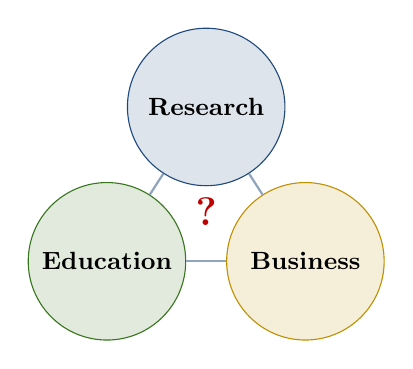
\begin{tikzpicture}[scale=0.7]
        \node[circle, draw=KaoBlue, fill=KaoBlue!15, minimum size=2cm, font=\small\bfseries] (R) at (0,2.3) {Research};
        \node[circle, draw=KaoGreen, fill=KaoGreen!15, minimum size=2cm, font=\small\bfseries] (E) at (-1.8,-0.5) {Education};
        \node[circle, draw=KaoGold, fill=KaoGold!15, minimum size=2cm, font=\small\bfseries] (B) at (1.8,-0.5) {Business};
        \draw[thick, KaoBlue!50] (R) -- (E);
        \draw[thick, KaoBlue!50] (R) -- (B);
        \draw[thick, KaoBlue!50] (E) -- (B);
        \node[font=\Large\bfseries, color=KaoRed] at (0,0.4) {?};
    \end{tikzpicture}
    {\scriptsize The Knowledge Triangle mandate}
\end{column}
\end{columns}
\note{Sustainability transitions require intermediaries. The EIT created 8 KICs to integrate the Knowledge Triangle. But we lack methods to map what these actors actually do.}
\end{frame}

% SLIDE 3: CARTOGRAPHIC GAP
\begin{frame}{The Cartographic Gap}
\secmark{Opening}
\begin{columns}[T]
\begin{column}{0.55\textwidth}
    \textbf{Existing approaches} study roles through:
    \begin{itemize}
        \item Single data sources (interviews, surveys)
        \item Single modalities (text \emph{or} networks \emph{or} images)
        \item Single theoretical lenses
    \end{itemize}
    \vspace{0.8em}
    \textbf{What is missing:}
    \begin{itemize}
        \item \alert{No multimodal integration} across data types
        \item No computational infrastructure for replication
        \item No systematic way to compare claimed vs.\ enacted roles
    \end{itemize}
\end{column}
\begin{column}{0.4\textwidth}
    \centering
    \begin{tikzpicture}[
        box/.style={rectangle, rounded corners=3pt, draw, minimum width=2.2cm, minimum height=0.55cm, font=\scriptsize, fill=#1!12, draw=#1},
        gap/.style={font=\scriptsize\bfseries, color=KaoRed}
    ]
        \node[box=KaoBlue] (w) at (0, 2) {\iconweb\ Websites};
        \node[box=KaoCyan] (s) at (0, 1.2) {\iconsocial\ Social};
        \node[box=KaoGold] (i) at (0, 0.4) {\iconinvest\ Investment};
        \node[box=KaoPurple] (v) at (0,-0.4) {\iconvisual\ Visual};
        \node[box=KaoGreen] (n) at (0,-1.2) {\iconnews\ News};
        \node[gap] at (2.5, 0.4) {Disconnected};
        \node[gap] at (2.5,-0.1) {silos};
        \draw[->, KaoRed, thick, dashed] (w.east) -- ++(0.8,0);
        \draw[->, KaoRed, thick, dashed] (s.east) -- ++(0.8,0);
        \draw[->, KaoRed, thick, dashed] (i.east) -- ++(0.8,0);
        \draw[->, KaoRed, thick, dashed] (v.east) -- ++(0.8,0);
        \draw[->, KaoRed, thick, dashed] (n.east) -- ++(0.8,0);
    \end{tikzpicture}
\end{column}
\end{columns}
\note{Many partial maps but no integrated atlas. Each data source reveals different facets of organizational roles. This is the gap this dissertation fills.}
\end{frame}

\section{Problem \& Research Questions}

% SLIDE 4: EIT ECOSYSTEM
\begin{frame}{Empirical Setting: The EIT Ecosystem}
\secmark{Problem}
\begin{columns}[T]
\begin{column}{0.55\textwidth}
    \textbf{European Institute of Innovation \& Technology}
    \begin{itemize}
        \item 8 Knowledge and Innovation Communities (KICs)
        \item Mandate: integrate the Knowledge Triangle
        \item Largest EU innovation instrument (\texteuro\,3B+)
    \end{itemize}
    \vspace{0.5em}
    {\small \textbf{KICs:} Climate, Digital, Food, Health, InnoEnergy, Manufacturing, Raw Materials, Urban Mobility}
\end{column}
\begin{column}{0.4\textwidth}
    \centering
    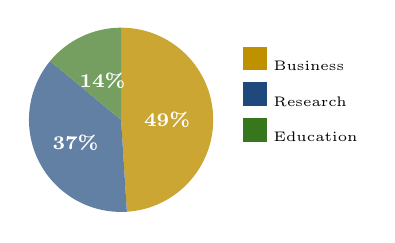
\begin{tikzpicture}[scale=0.65]
        \fill[KaoGold!80] (0,0) -- (90:1.8) arc (90:-86.4:1.8) -- cycle;
        \fill[KaoBlue!70] (0,0) -- (-86.4:1.8) arc (-86.4:-219.6:1.8) -- cycle;
        \fill[KaoGreen!70] (0,0) -- (-219.6:1.8) arc (-219.6:-270:1.8) -- cycle;
        \node[font=\scriptsize\bfseries, text=white] at (0:0.9) {49\%};
        \node[font=\scriptsize\bfseries, text=white] at (-153:1.0) {37\%};
        \node[font=\scriptsize\bfseries, text=white] at (-244.8:0.85) {14\%};
        \node[font=\tiny, anchor=west] at (2.2, 1.2) {\textcolor{KaoGold}{\rule{0.3cm}{0.3cm}} Business};
        \node[font=\tiny, anchor=west] at (2.2, 0.5) {\textcolor{KaoBlue}{\rule{0.3cm}{0.3cm}} Research};
        \node[font=\tiny, anchor=west] at (2.2,-0.2) {\textcolor{KaoGreen}{\rule{0.3cm}{0.3cm}} Education};
    \end{tikzpicture}
    {\scriptsize Knowledge Triangle ($n=1{,}298$)}
    \vspace{0.3em}
    {\scriptsize \alert{Business-dominant} despite balanced mandate}
\end{column}
\end{columns}
\note{The Knowledge Triangle imbalance is a key finding: business 49\%, research 37\%, education only 14\%. This challenges the balanced integration mandate of the EIT.}
\end{frame}

% SLIDE 5: MAIN RQ
\begin{frame}{Main Research Question}
\secmark{Problem}
\begin{center}
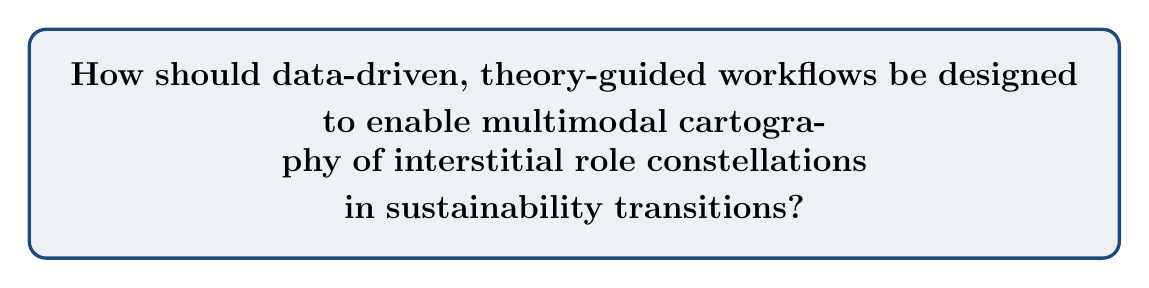
\begin{tikzpicture}
    \node[rectangle, rounded corners=6pt, draw=KaoBlue, fill=KaoBlue!8, line width=1.2pt, text width=13cm, align=center, inner sep=12pt, font=\large] {
        \textbf{How should data-driven, theory-guided workflows be designed\\[3pt]
        to enable multimodal cartography of interstitial role constellations\\[3pt]
        in sustainability transitions?}
    };
\end{tikzpicture}
\end{center}
\vspace{0.5em}
\small
\begin{description}[leftmargin=2.5cm]
    \item[Data-driven] Computational pipelines processing large-scale digital traces
    \item[Theory-guided] Grounded in role theory, sustainability transitions, sociomateriality
    \item[Multimodal] Six data modalities triangulated for convergence \emph{and} divergence
    \item[Interstitial] Organizations occupying spaces \emph{between} established fields
\end{description}
\note{This is a design science question: how to design workflows. Multimodal means combining data types, not just collecting more data.}
\end{frame}

% SLIDE 6: FOUR SUB-QUESTIONS
\begin{frame}{Four Sub-Questions}
\secmark{Problem}
\renewcommand{\arraystretch}{1.6}
\begin{tabularx}{\textwidth}{@{}l X l@{}}
\toprule
& \textbf{Research Question} & \textbf{Chapters} \\
\midrule
\textbf{RQ1} & \textit{Theory:} What framework enables theory-guided, empirically open analysis? & Ch.~2, 4 \\
\textbf{RQ2} & \textit{Method:} What methodology enables cross-modal mapping? & Ch.~3 \\
\textbf{RQ3} & \textit{Empirics:} What role patterns emerge in the EIT ecosystem? & Ch.~5--9 \\
\textbf{RQ4} & \textit{Implications:} How can DSR workflows break down open science barriers while building up research infrastructure? & Ch.~10, 12 \\
\bottomrule
\end{tabularx}
\note{RQ1 = theoretical. RQ2 = methodological. RQ3 = empirical. RQ4 = practical.}
\end{frame}

\section{Methodology}

% SLIDE 7: DSR
\begin{frame}{Design Science Research}
\secmark{Methodology}
\begin{columns}[T]
\begin{column}{0.5\textwidth}
    \textbf{DSR Paradigm} (Hevner et al.\ 2004)
    \begin{itemize}
        \item Build and evaluate \textbf{artifacts}
        \item Solve real-world design problems
        \item Produce \textbf{design knowledge}
    \end{itemize}
    \vspace{0.8em}
    \textbf{Metatheoretical grounding:}
    \begin{itemize}
        \item DSR = methodology
        \item Sociomateriality = ontology (Orlikowski 2007)
        \item Sustainability transitions = domain theory
    \end{itemize}
\end{column}
\begin{column}{0.45\textwidth}
    \centering
    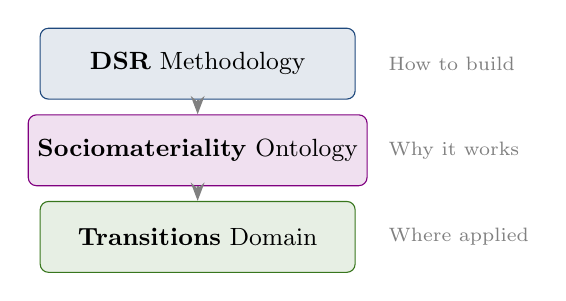
\begin{tikzpicture}[
        layer/.style={rectangle, rounded corners=3pt, draw=#1, fill=#1!12, minimum width=4cm, minimum height=0.9cm, font=\small},
    ]
        \node[layer=KaoBlue] (dsr) at (0,2.2) {\textbf{DSR} Methodology};
        \node[layer=KaoPurple] (sm) at (0,1.1) {\textbf{Sociomateriality} Ontology};
        \node[layer=KaoGreen] (st) at (0,0) {\textbf{Transitions} Domain};
        \draw[-{Stealth}, thick, gray] (dsr.south) -- (sm.north);
        \draw[-{Stealth}, thick, gray] (sm.south) -- (st.north);
        \node[font=\scriptsize, color=gray, anchor=west] at (2.3,2.2) {How to build};
        \node[font=\scriptsize, color=gray, anchor=west] at (2.3,1.1) {Why it works};
        \node[font=\scriptsize, color=gray, anchor=west] at (2.3,0) {Where applied};
    \end{tikzpicture}
\end{column}
\end{columns}
\note{Three-layer architecture. DSR is the methodology, sociomateriality explains why different modalities produce different but equally real role profiles, sustainability transitions is the empirical domain.}
\end{frame}

% SLIDE 8: MAASS FRAMEWORK
\begin{frame}{The Maass Bridging Framework}
\secmark{Methodology}
\centering
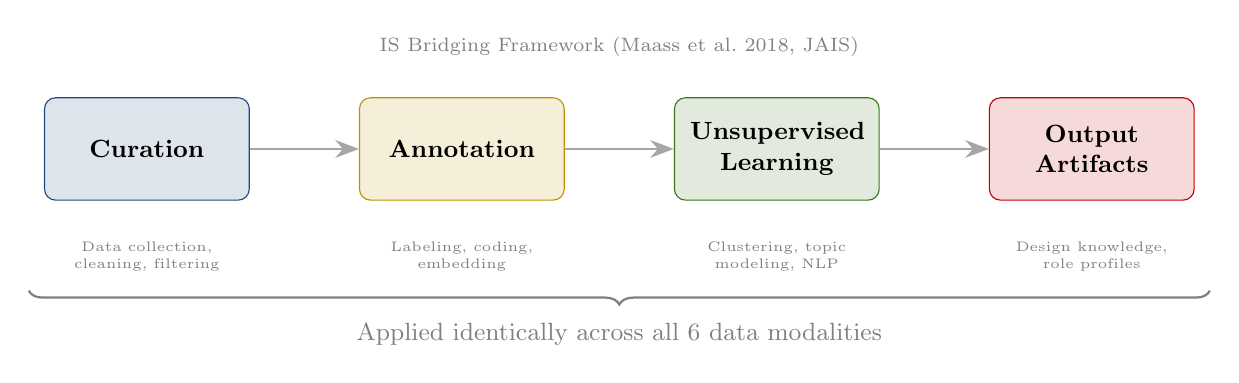
\begin{tikzpicture}[
    stage/.style={rectangle, rounded corners=4pt, draw=#1, fill=#1!15, minimum width=2.6cm, minimum height=1.3cm, font=\small\bfseries, text width=2.2cm, align=center},
    arr/.style={-{Stealth[length=3mm]}, thick, gray!70},
    lbl/.style={font=\tiny, color=gray, text width=2.4cm, align=center}
]
    \node[stage=KaoBlue]  (cur) at (0,0)  {Curation};
    \node[stage=KaoGold]  (ann) at (4,0)  {Annotation};
    \node[stage=KaoGreen] (uns) at (8,0)  {Unsupervised\\Learning};
    \node[stage=KaoRed]   (out) at (12,0) {Output\\Artifacts};
    \draw[arr] (cur) -- (ann);
    \draw[arr] (ann) -- (uns);
    \draw[arr] (uns) -- (out);
    \node[lbl, below=0.4cm of cur] {Data collection,\\cleaning, filtering};
    \node[lbl, below=0.4cm of ann] {Labeling, coding,\\embedding};
    \node[lbl, below=0.4cm of uns] {Clustering, topic\\modeling, NLP};
    \node[lbl, below=0.4cm of out] {Design knowledge,\\role profiles};
    \node[font=\scriptsize, color=gray] at (6, 1.3) {IS Bridging Framework (Maass et al.\ 2018, JAIS)};
    \draw[decorate, decoration={brace, amplitude=5pt, mirror}, thick, gray]
        (-1.5,-1.8) -- (13.5,-1.8)
        node[midway, below=8pt, font=\small] {Applied identically across all 6 data modalities};
\end{tikzpicture}
\note{The Maass bridging framework structures every empirical chapter identically. Big Data meets domain theory through four stages.}
\end{frame}

% SLIDE 9: ROLEBOX
\begin{frame}{\RoleBox{} Toolkit Architecture}
\secmark{Methodology}
\begin{columns}[T]
\begin{column}{0.5\textwidth}
    \textbf{Core artifact:} open-source computational toolkit
    \vspace{0.5em}
    \textbf{6 data modules:}
    \begin{enumerate}
        \item[\iconweb]     \textbf{Websites} --- 675 crawled sites
        \item[\iconsocial]  \textbf{Twitter/X} --- 268K tweets
        \item[\iconinvest]  \textbf{Crunchbase} --- 7,341 ventures
        \item[\iconvisual]  \textbf{Images} --- 31,508 visuals
        \item[\iconnews]    \textbf{News} --- 1,273 articles
        \item[\faBook]      \textbf{Wikipedia} --- EIT entity pages
    \end{enumerate}
\end{column}
\begin{column}{0.45\textwidth}
    \textbf{Meta-Design Requirements:}
    \begin{description}
        \item[MDR-1] Theory-guided curation
        \item[MDR-2] Cross-modal comparability
        \item[MDR-3] Reproducible pipelines
        \item[MDR-4] Open science infrastructure
    \end{description}
    \vspace{0.5em}
    \textbf{Outputs:}
    \begin{itemize}
        \item Role constellation maps
        \item Sociotype classifications
        \item Cross-modal gap metrics
    \end{itemize}
\end{column}
\end{columns}
\note{RoleBox is the central DSR artifact. Six git submodules, each implementing the Maass pipeline.}
\end{frame}

% SLIDE 10: SIX MODALITIES
\begin{frame}{Six Modalities, Five Role Views}
\secmark{Methodology}
\centering
\begin{tikzpicture}[
    mod/.style={rectangle, rounded corners=3pt, draw=#1, fill=#1!12, minimum width=2.4cm, minimum height=0.7cm, font=\small},
    view/.style={font=\small\itshape, color=gray!80},
    arr/.style={-{Stealth}, thick, #1!60}
]
    \node[mod=KaoBlue]   (web) at (-3, 2) {\iconweb\ Websites};
    \node[mod=KaoCyan]   (soc) at (-3, 1) {\iconsocial\ Social};
    \node[mod=KaoGold]   (inv) at (-3, 0) {\iconinvest\ Investment};
    \node[mod=KaoPurple] (vis) at (-3,-1) {\iconvisual\ Visual};
    \node[mod=KaoGreen]  (new) at (-3,-2) {\iconnews\ News};
    \node[view] (cv) at (3, 2) {Claimed roles};
    \node[view] (rv) at (3, 1) {Relational roles};
    \node[view] (iv) at (3, 0) {Resourced roles};
    \node[view] (ev) at (3,-1) {Embodied roles};
    \node[view] (av) at (3,-2) {Attributed roles};
    \draw[arr=KaoBlue]   (web) -- (cv);
    \draw[arr=KaoCyan]   (soc) -- (rv);
    \draw[arr=KaoGold]   (inv) -- (iv);
    \draw[arr=KaoPurple] (vis) -- (ev);
    \draw[arr=KaoGreen]  (new) -- (av);
    \node[circle, draw=KaoRed, fill=KaoRed!10, minimum size=1.2cm, font=\scriptsize\bfseries, text width=1cm, align=center] (int) at (6.5, 0) {Role\\Profile};
    \foreach \v in {cv, rv, iv, ev, av} {
        \draw[-{Stealth}, thick, KaoRed!40] (\v.east) -- (int.west);
    }
\end{tikzpicture}
\vspace{0.3em}
{\small Each modality reveals a \textbf{different facet} of the same organization.\\
Convergence validates; \alert{divergence} reveals tensions and aspirations.}
\note{Core conceptual diagram. Sociomateriality explains why modalities diverge.}
\end{frame}

\section{Empirical Findings}

% SLIDE 11: CH.5
\begin{frame}{Ch.~5: Interstitial Pluralism --- Wikipedia \& Websites}
\secmark{Empirics: Claimed Roles}
\begin{columns}[T]
\begin{column}{0.45\textwidth}
    \textbf{\faDatabase\ Data \& Method}
    \begin{itemize}
        \item 675 crawled EIT partner websites
        \item Wikipedia entity descriptions
        \item NLP: topic modeling, embeddings
        \item Sociotype classification
    \end{itemize}
    \vspace{0.5em}
    \textbf{\faCogs\ Pipeline}\\
    {\small Curation $\to$ Text extraction $\to$ Embedding $\to$ Clustering}
\end{column}
\begin{column}{0.5\textwidth}
    \textbf{\faLightbulb[regular]\ Key Findings}
    \begin{itemize}
        \item \textbf{5 website sociotypes} identified
        \item Organizations claim multiple roles simultaneously
        \item ``Interstitial pluralism'': strategic ambiguity as a feature
        \item Knowledge Triangle imbalance visible in self-descriptions
    \end{itemize}
    \vspace{0.3em}
    \begin{block}{\scriptsize Insight}
        \scriptsize Organizations \emph{between} fields adopt plural identities that resist single-category classification.
    \end{block}
\end{column}
\end{columns}
\note{Ch.5 introduces interstitial pluralism. Five sociotypes emerge from website text.}
\end{frame}

% SLIDE 12: SOCIOTYPES
\begin{frame}{Five Website Sociotypes}
\secmark{Empirics: Claimed Roles}
\centering
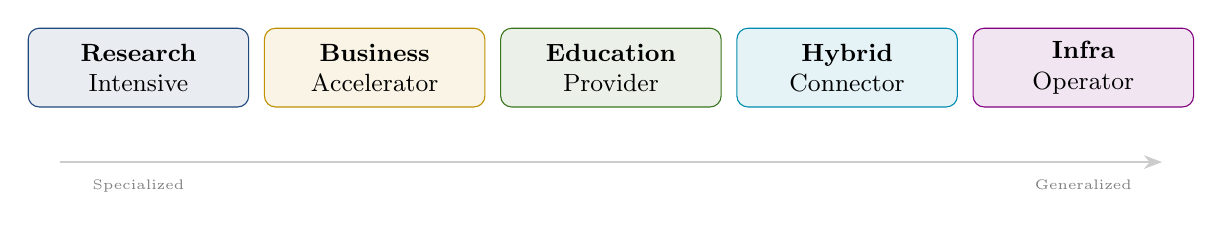
\begin{tikzpicture}[
    stype/.style={rectangle, rounded corners=4pt, draw=#1, fill=#1!10, minimum width=2.8cm, minimum height=1cm, font=\small, text width=2.5cm, align=center}
]
    \node[stype=KaoBlue]   at (-5, 0) {\textbf{Research}\\Intensive};
    \node[stype=KaoGold]   at (-2, 0) {\textbf{Business}\\Accelerator};
    \node[stype=KaoGreen]  at ( 1, 0) {\textbf{Education}\\Provider};
    \node[stype=KaoCyan]   at ( 4, 0) {\textbf{Hybrid}\\Connector};
    \node[stype=KaoPurple] at ( 7, 0) {\textbf{Infra}\\Operator};
    \draw[-{Stealth}, gray!40, thick] (-6, -1.2) -- (8, -1.2);
    \node[font=\tiny, color=gray, anchor=north] at (-5, -1.3) {Specialized};
    \node[font=\tiny, color=gray, anchor=north] at ( 7, -1.3) {Generalized};
\end{tikzpicture}
\vspace{1em}
{\small
\begin{itemize}
    \item Sociotypes are \textbf{cross-modal constructs}: no single data source reveals them all
    \item The \textbf{Hybrid Connector} type is the most prevalent---and the most aspirational
    \item Sociotype membership correlates with KIC domain and organizational age
\end{itemize}
}
\note{Hybrid Connectors are the most common claimed identity. Later chapters show many claims are aspirational.}
\end{frame}

% SLIDE 13: CH.6
\begin{frame}{Ch.~6: The Rolefield --- Twitter Curation Networks}
\secmark{Empirics: Relational Roles}
\begin{columns}[T]
\begin{column}{0.45\textwidth}
    \textbf{\faDatabase\ Data \& Method}
    \begin{itemize}
        \item 268,000 tweets from EIT ecosystem
        \item 500 actors, 96 communities
        \item Twitter list co-classification
        \item Network analysis (modularity, centrality)
    \end{itemize}
    \vspace{0.5em}
    \textbf{4 structural roles:}\\
    {\small Hub $\cdot$ Bridge $\cdot$ Amplifier $\cdot$ Receiver}
\end{column}
\begin{column}{0.5\textwidth}
    \textbf{\faLightbulb[regular]\ Key Findings}
    \begin{itemize}
        \item \textbf{8 major community clusters}
        \item KICs act as \textbf{hubs} within domains but \textbf{weak bridges} across domains
        \item Role specialization varies by KIC maturity
        \item Curation networks reveal field structure invisible in follower networks
    \end{itemize}
    \vspace{0.3em}
    \begin{block}{\scriptsize Insight}
        \scriptsize Twitter \emph{lists} (curation) reveal deliberate classification acts, unlike passive following.
    \end{block}
\end{column}
\end{columns}
\note{Ch.6 introduces the rolefield concept. Twitter lists are curation acts.}
\end{frame}

% SLIDE 14: STRUCTURAL ROLES
\begin{frame}{Four Structural Roles in the Rolefield}
\secmark{Empirics: Relational Roles}
\centering
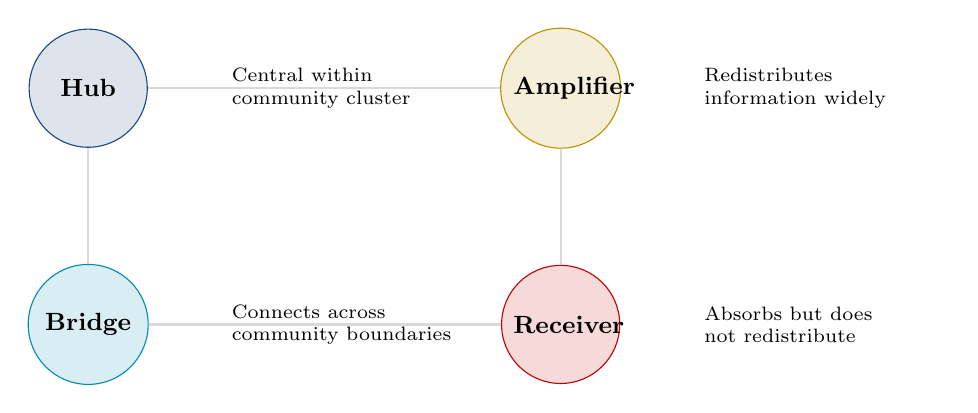
\begin{tikzpicture}[
    role/.style={circle, draw=#1, fill=#1!15, minimum size=1.5cm, font=\small\bfseries, text width=1.2cm, align=center},
    desc/.style={font=\scriptsize, text width=3cm, align=left, anchor=west}
]
    \node[role=KaoBlue] (hub) at (-4, 1.5) {Hub};
    \node[role=KaoCyan] (bri) at (-4,-1.5) {Bridge};
    \node[role=KaoGold] (amp) at ( 2, 1.5) {Amplifier};
    \node[role=KaoRed]  (rec) at ( 2,-1.5) {Receiver};
    \node[desc] at (-2.3, 1.5) {Central within\\community cluster};
    \node[desc] at (-2.3,-1.5) {Connects across\\community boundaries};
    \node[desc] at ( 3.7, 1.5) {Redistributes\\information widely};
    \node[desc] at ( 3.7,-1.5) {Absorbs but does\\not redistribute};
    \draw[thick, gray!30] (hub) -- (bri);
    \draw[thick, gray!30] (hub) -- (amp);
    \draw[thick, gray!30] (bri) -- (rec);
    \draw[thick, gray!30] (amp) -- (rec);
\end{tikzpicture}
\vspace{0.5em}
{\small KICs are strong \textbf{Hubs} but weak \textbf{Bridges}---they concentrate rather than distribute connectivity.}
\note{The key tension: KICs are central within their domain but poor at bridging across domains. This is the structural basis of the connector gap.}
\end{frame}

% SLIDE 15: CH.7
\begin{frame}{Ch.~7: Venture Positioning --- Crunchbase}
\secmark{Empirics: Resourced Roles}
\begin{columns}[T]
\begin{column}{0.45\textwidth}
    \textbf{\faDatabase\ Data \& Method}
    \begin{itemize}
        \item 7,341 sector ventures
        \item 654 direct EIT ventures
        \item Crunchbase funding data
        \item Sector embedding + clustering
    \end{itemize}
    \vspace{0.5em}
    \textbf{\faCogs\ Pipeline}\\
    {\small API harvest $\to$ Description embedding $\to$ UMAP $\to$ Sector maps}
\end{column}
\begin{column}{0.5\textwidth}
    \textbf{\faLightbulb[regular]\ Key Findings}
    \begin{itemize}
        \item EIT ventures cluster in \textbf{cleantech}, \textbf{health-tech}, \textbf{agri-food}
        \item Business-dominant: 49\% of KT entities
        \item Funding reveals \textbf{enacted} (not claimed) priorities
        \item Gap between KIC labels and actual venture portfolios
    \end{itemize}
    \vspace{0.3em}
    \begin{block}{\scriptsize Insight}
        \scriptsize Investment records show what organizations \emph{fund}, not what they \emph{say}.
    \end{block}
\end{column}
\end{columns}
\note{Ch.7 uses Crunchbase as a revealed-preference measure. Business-dominant KT (49\%) is clearest here.}
\end{frame}

% SLIDE 16: CH.8
\begin{frame}{Ch.~8: Visual Registers --- Image Analysis}
\secmark{Empirics: Embodied Roles}
\begin{columns}[T]
\begin{column}{0.45\textwidth}
    \textbf{\faDatabase\ Data \& Method}
    \begin{itemize}
        \item 31,508 deduplicated images
        \item 2,003 hand-coded images
        \item DINOv2 + LLaVA/BLIP embeddings
        \item Visual register classification
    \end{itemize}
    \vspace{0.5em}
    \textbf{\faCogs\ Pipeline}\\
    {\small Collection $\to$ Dedup $\to$ Embedding $\to$ Register coding}
\end{column}
\begin{column}{0.5\textwidth}
    \textbf{\faLightbulb[regular]\ Key Findings}
    \begin{itemize}
        \item Distinct \textbf{visual registers} per KIC
        \item Technology images dominate over people images
        \item Visual identity reinforces or contradicts textual claims
        \item Visual rhetoric of connectivity
    \end{itemize}
    \vspace{0.3em}
    \begin{block}{\scriptsize Insight}
        \scriptsize Images perform roles that text cannot: they make institutional identity \emph{visible} and \emph{embodied}.
    \end{block}
\end{column}
\end{columns}
\note{31K images is one of the largest visual corpora in transition studies.}
\end{frame}

% SLIDE 17: CH.9
\begin{frame}{Ch.~9: Power \& Agency --- News Discourse}
\secmark{Empirics: Attributed Roles}
\begin{columns}[T]
\begin{column}{0.45\textwidth}
    \textbf{\faDatabase\ Data \& Method}
    \begin{itemize}
        \item 1,273 news articles
        \item 33,484 semantic triples (S-V-O)
        \item RIVETER-X NLP pipeline
        \item Connotation frames analysis
    \end{itemize}
    \vspace{0.5em}
    \textbf{\faCogs\ Pipeline}\\
    {\small Harvest $\to$ NER $\to$ SRL $\to$ Verb frames $\to$ Agency scores}
\end{column}
\begin{column}{0.5\textwidth}
    \textbf{\faLightbulb[regular]\ Key Findings}
    \begin{itemize}
        \item \textbf{Agency hierarchy}: EU institutions at top, startups at bottom
        \item KICs positioned as \textbf{instruments}, not autonomous agents
        \item Verb analysis reveals power asymmetries
        \item News media \emph{constructs} roles through discourse
    \end{itemize}
    \vspace{0.3em}
    \begin{block}{\scriptsize Insight}
        \scriptsize Discourse does not just \emph{describe} power---it \emph{performs} it through verb choice and subject positioning.
    \end{block}
\end{column}
\end{columns}
\note{KICs are more often objects than subjects in news discourse. Contrasts with self-presentation on websites.}
\end{frame}

% SLIDE 18: AGENCY HIERARCHY
\begin{frame}{The Agency Hierarchy}
\secmark{Empirics: Attributed Roles}
\centering
\begin{tikzpicture}[
    level/.style={rectangle, rounded corners=3pt, draw=#1, fill=#1!12, minimum height=0.7cm, font=\small, text width=#2, align=center}
]
    \node[level=KaoBlue{4cm}]   at (0, 3)   {\textbf{EU Institutions}};
    \node[level=KaoCyan{5.5cm}] at (0, 2)   {National Governments};
    \node[level=KaoGold{7cm}]   at (0, 1)   {EIT \& KICs (intermediaries)};
    \node[level=KaoGreen{8.5cm}] at (0, 0)   {Universities \& Research Centres};
    \node[level=KaoRed{10cm}]   at (0,-1)   {Startups \& SMEs};
    \node[font=\scriptsize\bfseries, color=KaoBlue, anchor=east] at (-5.5, 3) {High agency};
    \node[font=\scriptsize\bfseries, color=KaoRed, anchor=east] at (-5.5,-1) {Low agency};
    \draw[-{Stealth}, thick, gray!50] (-5.5, 2.5) -- (-5.5, -0.5);
    \node[font=\tiny, color=gray, anchor=west] at (2.3, 3) {``fund,'' ``mandate,'' ``establish''};
    \node[font=\tiny, color=gray, anchor=west] at (4, 1) {``coordinate,'' ``support''};
    \node[font=\tiny, color=gray, anchor=west] at (5.5, -1) {``receive,'' ``benefit,'' ``participate''};
\end{tikzpicture}
\vspace{0.5em}
{\small Verb choice in news discourse constructs a \alert{power gradient} where intermediaries are \emph{instruments} of higher-agency actors.}
\note{EU institutions use high-agency verbs (fund, mandate). Startups use low-agency verbs (receive, benefit). KICs sit in the middle.}
\end{frame}

% SLIDE 19: CONNECTOR GAP
\begin{frame}{The Connector Gap: Convergence and Divergence}
\secmark{Empirics: Synthesis}
\begin{columns}[T]
\begin{column}{0.5\textwidth}
    \textbf{Three convergent findings across modalities:}
    \begin{enumerate}
        \item \alert{Connector gap}: 34\% claim connector roles, only 13\% enact them (21-point gap)
        \item \alert{KT imbalance}: Business 49\%, Research 37\%, Education 14\%
        \item \alert{Five sociotypes}: invisible to any single modality alone
    \end{enumerate}
    \vspace{0.5em}
    {\small \textbf{Sociomaterial explanation:} Platforms \emph{co-constitute} different role realities.}
\end{column}
\begin{column}{0.45\textwidth}
    \centering
    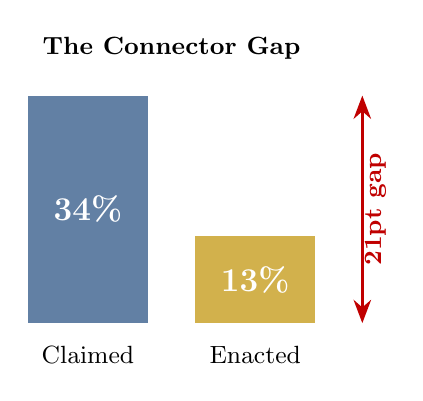
\begin{tikzpicture}[scale=0.85]
        \fill[KaoBlue!70] (0,0) rectangle (1.8,3.4);
        \fill[KaoGold!70] (2.5,0) rectangle (4.3,1.3);
        \node[font=\small, anchor=north] at (0.9,-0.2) {Claimed};
        \node[font=\small, anchor=north] at (3.4,-0.2) {Enacted};
        \node[font=\large\bfseries, text=white] at (0.9,1.7) {34\%};
        \node[font=\large\bfseries, text=white] at (3.4,0.65) {13\%};
        \draw[{Stealth}-{Stealth}, line width=1.2pt, KaoRed] (5,0) -- (5,3.4);
        \node[font=\small\bfseries, text=KaoRed, rotate=90, anchor=south] at (5.5,1.7) {21pt gap};
        \node[font=\small\bfseries, anchor=south] at (2.15,3.8) {The Connector Gap};
    \end{tikzpicture}
\end{column}
\end{columns}
\note{The connector gap is the headline finding. Reproduced across all 8 KIC domains.}
\end{frame}

\section{Transferability}

% SLIDE 20: VIDEO
\begin{frame}{Ch.~11: The Seventh Modality --- Video Workflows}
\secmark{Transferability}
\begin{columns}[T]
\begin{column}{0.5\textwidth}
    \textbf{Demonstrating transferability:}
    \begin{itemize}
        \item \RoleBox{} pipeline applied to \textbf{video} data
        \item Three tools: Masked-Piper, MaskAnyone, AMP Pipeline
        \item Same Maass framework: Curation $\to$ Annotation $\to$ Unsupervised $\to$ Output
    \end{itemize}
    \vspace{0.5em}
    \textbf{Key point:}\\
    {\small The workflow architecture generalizes beyond the 5 empirical modalities---it is \alert{modality-agnostic}.}
\end{column}
\begin{column}{0.45\textwidth}
    \centering
    \begin{tikzpicture}[
        tool/.style={rectangle, rounded corners=3pt, draw=KaoPurple, fill=KaoPurple!10, minimum width=3cm, minimum height=0.7cm, font=\small}
    ]
        \node[tool] (mp)  at (0, 1.5) {\faVideo\ Masked-Piper};
        \node[tool] (ma)  at (0, 0.5) {\faUserSecret\ MaskAnyone};
        \node[tool] (amp) at (0,-0.5) {\faCogs\ AMP Pipeline};
        \node[rectangle, rounded corners=3pt, draw=KaoGreen, fill=KaoGreen!10, minimum width=3cm, minimum height=0.7cm, font=\small\bfseries] (out) at (0,-1.7) {Video Role Maps};
        \draw[-{Stealth}, thick, gray] (mp.south)  -- (ma.north);
        \draw[-{Stealth}, thick, gray] (ma.south)  -- (amp.north);
        \draw[-{Stealth}, thick, gray] (amp.south) -- (out.north);
    \end{tikzpicture}
    \vspace{0.3em}
    {\scriptsize 7th modality --- transferability demonstration}
\end{column}
\end{columns}
\note{If the pipeline works for video, the architecture is truly generalizable.}
\end{frame}

\section{Contributions}

% SLIDE 21: SOCIOTYPE FRAMEWORK
\begin{frame}{Contribution 1: The Sociotype Framework}
\secmark{Contributions}
\begin{columns}[T]
\begin{column}{0.55\textwidth}
    \textbf{What is a sociotype?}
    \begin{itemize}
        \item A \textbf{multimodal role profile} synthesized across data sources
        \item Goes beyond single-modality typologies
        \item Captures both claimed and enacted roles
    \end{itemize}
    \vspace{0.5em}
    \textbf{Five sociotypes identified:}
    \begin{enumerate}
        \item Research-intensive partners
        \item Business accelerators
        \item Education providers
        \item Hybrid connectors
        \item Infrastructure operators
    \end{enumerate}
\end{column}
\begin{column}{0.4\textwidth}
    \centering
    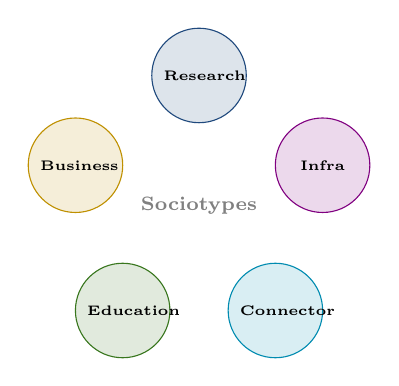
\begin{tikzpicture}[scale=0.75]
        \foreach \i/\lab/\col in {1/Research/KaoBlue, 2/Business/KaoGold, 3/Education/KaoGreen, 4/Connector/KaoCyan, 5/Infra/KaoPurple} {
            \node[circle, draw=\col, fill=\col!15, minimum size=1.2cm, font=\tiny\bfseries, text width=0.9cm, align=center] at ({90+(\i-1)*72}:2.2) {\lab};
        }
        \node[font=\scriptsize\bfseries, color=gray] at (0,0) {Sociotypes};
    \end{tikzpicture}
\end{column}
\end{columns}
\note{The sociotype framework integrates role signals from all five modalities into a unified typology.}
\end{frame}

% SLIDE 22: MULTIMODAL CARTOGRAPHY
\begin{frame}{Contribution 2: Multimodal Cartography as IS Bridging Research}
\secmark{Contributions}
\begin{columns}[T]
\begin{column}{0.55\textwidth}
    \textbf{Methodological contribution:}
    \begin{itemize}
        \item Replicable pipeline architecture
        \item Each modality follows identical 4-stage framework
        \item Cross-modal integration produces design knowledge
    \end{itemize}
    \vspace{0.5em}
    \textbf{What makes it ``bridging'':}
    \begin{itemize}
        \item Big Data $\leftrightarrow$ Domain Theory
        \item Computational methods $\leftrightarrow$ Interpretive framing
        \item Open infrastructure $\leftrightarrow$ Academic contribution
    \end{itemize}
\end{column}
\begin{column}{0.4\textwidth}
    \centering
    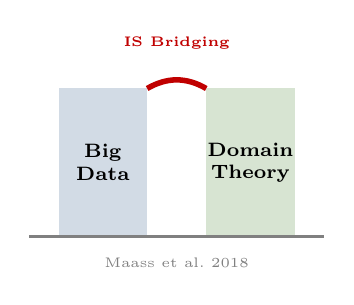
\begin{tikzpicture}[scale=0.75]
        \fill[KaoBlue!20] (-2, 0) rectangle (-0.5, 2.5);
        \fill[KaoGreen!20] (0.5, 0) rectangle (2, 2.5);
        \node[font=\scriptsize\bfseries, text width=1.3cm, align=center] at (-1.25, 1.25) {Big\\Data};
        \node[font=\scriptsize\bfseries, text width=1.3cm, align=center] at (1.25, 1.25) {Domain\\Theory};
        \draw[line width=2pt, KaoRed] (-0.5, 2.5) to[out=30, in=150] (0.5, 2.5);
        \node[font=\tiny\bfseries, color=KaoRed, anchor=south] at (0, 3) {IS Bridging};
        \draw[line width=1pt, gray] (-2.5, 0) -- (2.5, 0);
        \node[font=\tiny, color=gray, anchor=north] at (0, -0.2) {Maass et al.\ 2018};
    \end{tikzpicture}
\end{column}
\end{columns}
\note{The contribution is not just findings but a reusable pipeline architecture.}
\end{frame}

% SLIDE 23: EMPIRICAL PATTERNS
\begin{frame}{Contribution 3: Empirical Patterns in the EIT Ecosystem}
\secmark{Contributions}
\textbf{Novel empirical findings about Europe's largest innovation ecosystem:}
\vspace{0.5em}
\renewcommand{\arraystretch}{1.3}
\begin{tabularx}{\textwidth}{@{}>{\bfseries}l X >{\small}r@{}}
\toprule
\textbf{Finding} & \textbf{Description} & \textbf{Source} \\
\midrule
Connector Gap  & 34\% claim vs.\ 13\% enact connector roles & Ch.~5+6 \\
KT Imbalance   & Business 49\%, Research 37\%, Education 14\% & Ch.~7 \\
Visual Registers & KICs deploy distinct visual identity strategies & Ch.~8 \\
Agency Hierarchy & EU institutions top, startups bottom & Ch.~9 \\
Sociotype Stability & Role profiles stable across 3+ modalities & Ch.~10 \\
\bottomrule
\end{tabularx}
\vspace{0.5em}
{\small These patterns are \textbf{only visible} through multimodal triangulation---no single data source reveals them.}
\note{Actionable findings for policymakers. The KT imbalance challenges EIT founding premise.}
\end{frame}

\section{Discussion}

% SLIDE 24: PROPOSITIONS
\begin{frame}{Five Propositions}
\secmark{Discussion}
\begin{enumerate}
    \item[\textbf{P1}] Interstitial organizations adopt \textbf{plural role identities} that vary systematically across data modalities
    \vspace{0.4em}
    \item[\textbf{P2}] The \textbf{connector gap} between claimed and enacted roles is a structural feature of intermediary ecosystems, not measurement error
    \vspace{0.4em}
    \item[\textbf{P3}] \textbf{Sociomaterial constitution}: different platforms produce different---but equally real---role realities
    \vspace{0.4em}
    \item[\textbf{P4}] \textbf{Multimodal cartography} produces design knowledge that single-modality studies cannot
    \vspace{0.4em}
    \item[\textbf{P5}] \textbf{DSR workflows} can function as cumulative open science infrastructure when designed with modularity and replicability
\end{enumerate}
\note{P1--P2 are empirical. P3 is theoretical. P4 is methodological. P5 is practical.}
\end{frame}

% SLIDE 25: LIMITATIONS
\begin{frame}{Limitations}
\secmark{Discussion}
\begin{columns}[T]
\begin{column}{0.48\textwidth}
    \textbf{Data limitations}
    \begin{itemize}
        \item Single ecosystem (EIT)---generalizability?
        \item Temporal snapshot (2019--2023)
        \item Platform dependencies (Twitter/X API changes)
        \item English-language bias in NLP pipelines
    \end{itemize}
\end{column}
\begin{column}{0.48\textwidth}
    \textbf{Methodological limitations}
    \begin{itemize}
        \item Computational proxies for ``roles''
        \item Unsupervised clustering requires interpretation
        \item Cross-modal weighting is theory-dependent
        \item Visual coding inter-rater reliability
    \end{itemize}
\end{column}
\end{columns}
\vspace{0.8em}
\textbf{Mitigations:} {\small Ch.~11 (video) demonstrates transferability. Open infrastructure enables replication and extension by others.}
\note{Be honest about limitations but frame them constructively.}
\end{frame}

% SLIDE 26: FUTURE
\begin{frame}{Future Research}
\secmark{Discussion}
\begin{columns}[T]
\begin{column}{0.48\textwidth}
    \textbf{Extending the framework}
    \begin{itemize}
        \item Longitudinal role dynamics
        \item Additional ecosystems (national, sectoral)
        \item Real-time dashboard monitoring
        \item LLM-augmented annotation
    \end{itemize}
\end{column}
\begin{column}{0.48\textwidth}
    \textbf{Deepening the theory}
    \begin{itemize}
        \item Role \emph{performance} vs.\ role \emph{structure}
        \item Agent-based modeling (\RoleSim)
        \item Institutional work and role change
        \item Platform governance implications
    \end{itemize}
\end{column}
\end{columns}
\vspace{0.8em}
\centering
\begin{tikzpicture}
    \node[rectangle, rounded corners=4pt, draw=KaoGreen, fill=KaoGreen!8, inner sep=8pt, font=\small] {
        \faGithub\ \ \textbf{Open infrastructure:} All pipelines, data modules, and workflows are publicly available
    };
\end{tikzpicture}
\note{Future work in two directions: extending to new contexts and deepening theory.}
\end{frame}

\section{Closing}

% SLIDE 27: SUMMARY
\begin{frame}{Summary: Multimodal Cartography of Role Constellations}
\secmark{Closing}
\centering
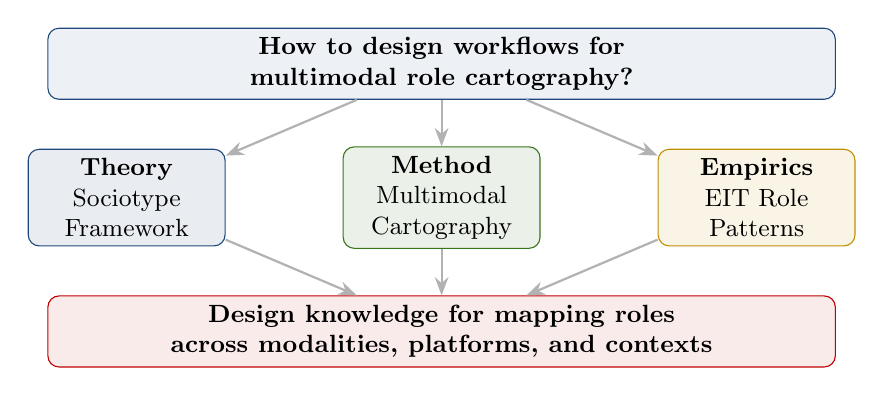
\begin{tikzpicture}[
    box/.style={rectangle, rounded corners=4pt, draw=#1, fill=#1!10, minimum width=2.5cm, minimum height=1cm, font=\small, text width=2.2cm, align=center},
    arr/.style={-{Stealth}, thick, gray!60}
]
    \node[rectangle, rounded corners=4pt, draw=KaoBlue, fill=KaoBlue!8, minimum width=10cm, minimum height=0.8cm, font=\small\bfseries, text width=9.5cm, align=center] (rq) at (0, 3.2) {How to design workflows for multimodal role cartography?};
    \node[box=KaoBlue]  (c1) at (-4, 1.5) {\textbf{Theory}\\Sociotype\\Framework};
    \node[box=KaoGreen] (c2) at ( 0, 1.5) {\textbf{Method}\\Multimodal\\Cartography};
    \node[box=KaoGold]  (c3) at ( 4, 1.5) {\textbf{Empirics}\\EIT Role\\Patterns};
    \node[rectangle, rounded corners=4pt, draw=KaoRed, fill=KaoRed!8, minimum width=10cm, minimum height=0.8cm, font=\small\bfseries, text width=9.5cm, align=center] (ans) at (0, -0.2) {Design knowledge for mapping roles across modalities, platforms, and contexts};
    \draw[arr] (rq) -- (c1);
    \draw[arr] (rq) -- (c2);
    \draw[arr] (rq) -- (c3);
    \draw[arr] (c1) -- (ans);
    \draw[arr] (c2) -- (ans);
    \draw[arr] (c3) -- (ans);
\end{tikzpicture}
\vspace{0.5em}
{\small 6 modalities $\cdot$ 8 KICs $\cdot$ 300K+ data points $\cdot$ 1 replicable framework}
\note{Three contributions answering one design science question. Not just analysis---reusable infrastructure.}
\end{frame}

% SLIDE 28: THANK YOU
\begin{frame}[standout]
    Thank you

    \vspace{1em}
    {\large Questions?}

    \vspace{1em}
    {\normalsize Babajide Alamu Owoyele}\\
    {\small DRIFT / Erasmus University Rotterdam}
\end{frame}

%========================================================================================
% BACKUP SLIDES
%========================================================================================
\appendix

\begin{frame}{Backup: Data Scale Summary}
\secmark{Appendix}
\centering
\renewcommand{\arraystretch}{1.3}
\begin{tabular}{@{}l l r l@{}}
\toprule
\textbf{Modality} & \textbf{Source} & \textbf{n} & \textbf{Chapter} \\
\midrule
\iconweb\ Websites     & EIT partner sites  & 675     & Ch.~5 \\
\iconsocial\ Social    & Twitter/X          & 268,000 & Ch.~6 \\
\iconinvest\ Investment& Crunchbase         & 7,341   & Ch.~7 \\
\iconvisual\ Visual    & Images             & 31,508  & Ch.~8 \\
\iconnews\ News        & Media articles     & 1,273   & Ch.~9 \\
\faBook\ Wikipedia     & Entity pages       & ---     & Ch.~5 \\
\iconvideo\ Video      & Transferability    & ---     & Ch.~11 \\
\bottomrule
\end{tabular}
\end{frame}

\begin{frame}{Backup: Meta-Design Requirements}
\secmark{Appendix}
\begin{description}
    \item[MDR-1] \textbf{Theory-guided curation:} Data collection guided by domain theory rather than convenience sampling
    \item[MDR-2] \textbf{Cross-modal comparability:} Workflows produce outputs that can be meaningfully compared across modalities
    \item[MDR-3] \textbf{Reproducible pipelines:} All computational steps documented, versioned, and executable by others
    \item[MDR-4] \textbf{Open science infrastructure:} Artifacts designed for cumulative use, not one-off analysis
\end{description}
\end{frame}

\begin{frame}{Backup: Sociomaterial Account of Divergence}
\secmark{Appendix}
\textbf{Why do modalities produce different role profiles?}
\vspace{0.5em}
\begin{enumerate}
    \item \textbf{Measurement error} --- different biases $\to$ random divergence\\
        {\small\color{gray} Rejected: the connector gap is systematic, not random}
    \item \textbf{Strategic behavior} --- impression management $\to$ deliberate divergence\\
        {\small\color{gray} Partial: captures something real but treats platforms as neutral}
    \item \textbf{Sociomaterial constitution} --- platform affordances co-produce roles\\
        {\small\color{gray} Adopted: platforms materially shape what aspects of roles become observable}
\end{enumerate}
\vspace{0.5em}
Following Orlikowski (2007): ``The social and the material are constitutively entangled in everyday life.''
\end{frame}

\begin{frame}{Backup: Role Categories (Ch.~2)}
\secmark{Appendix}
\begin{columns}[T]
\begin{column}{0.48\textwidth}
    \textbf{From the literature:}
    \begin{itemize}
        \item Role theory (Biddle 1986)
        \item Organizational roles (Katz \& Kahn)
        \item Intermediary typologies (Howells 2006)
        \item Complex Adaptive Systems
    \end{itemize}
\end{column}
\begin{column}{0.48\textwidth}
    \textbf{This dissertation's framework:}
    \begin{itemize}
        \item Roles as \emph{performed}, not \emph{fixed}
        \item Multiple roles co-exist
        \item Modality shapes observation
        \item Role constellations, not taxonomies
    \end{itemize}
\end{column}
\end{columns}
\end{frame}

\begin{frame}{Backup: Supervision Committee}
\secmark{Appendix}
\begin{description}
    \item[Promotor] Prof.\ dr.\ Derk Loorbach {\small (DRIFT / Erasmus University Rotterdam)}
    \item[Co-promotor] Prof.\ dr.\ Gerard de Melo
    \item[Co-promotor] Dr.\ Jonathan Antonio Edelman
\end{description}
\end{frame}

\begin{frame}{Backup: Dissertation Structure}
\secmark{Appendix}
\centering
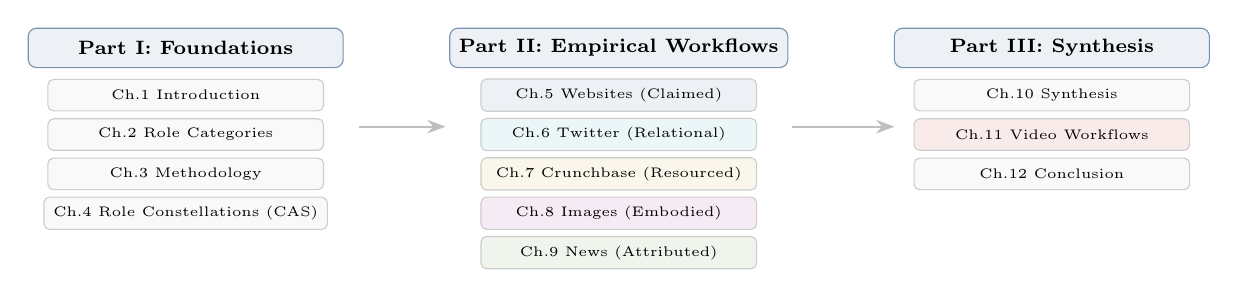
\begin{tikzpicture}[
    part/.style={rectangle, rounded corners=3pt, draw=KaoBlue!60, fill=KaoBlue!8, minimum width=4cm, minimum height=0.5cm, font=\scriptsize},
    ch/.style={rectangle, rounded corners=2pt, draw=gray!40, fill=gray!5, minimum width=3.5cm, minimum height=0.4cm, font=\tiny}
]
    \node[part, font=\scriptsize\bfseries] at (0, 3) {Part I: Foundations};
    \node[ch] at (0, 2.4) {Ch.1 Introduction};
    \node[ch] at (0, 1.9) {Ch.2 Role Categories};
    \node[ch] at (0, 1.4) {Ch.3 Methodology};
    \node[ch] at (0, 0.9) {Ch.4 Role Constellations (CAS)};
    \node[part, font=\scriptsize\bfseries] at (5.5, 3) {Part II: Empirical Workflows};
    \node[ch, fill=KaoBlue!8]   at (5.5, 2.4) {Ch.5 Websites (Claimed)};
    \node[ch, fill=KaoCyan!8]   at (5.5, 1.9) {Ch.6 Twitter (Relational)};
    \node[ch, fill=KaoGold!8]   at (5.5, 1.4) {Ch.7 Crunchbase (Resourced)};
    \node[ch, fill=KaoPurple!8] at (5.5, 0.9) {Ch.8 Images (Embodied)};
    \node[ch, fill=KaoGreen!8]  at (5.5, 0.4) {Ch.9 News (Attributed)};
    \node[part, font=\scriptsize\bfseries] at (11, 3) {Part III: Synthesis};
    \node[ch] at (11, 2.4) {Ch.10 Synthesis};
    \node[ch, fill=KaoRed!8] at (11, 1.9) {Ch.11 Video Workflows};
    \node[ch] at (11, 1.4) {Ch.12 Conclusion};
    \draw[-{Stealth}, thick, gray!50] (2.2, 2) -- (3.3, 2);
    \draw[-{Stealth}, thick, gray!50] (7.7, 2) -- (9, 2);
\end{tikzpicture}
\end{frame}

\end{document}
